\documentclass[]{article}

\usepackage{pdfpages,enumitem,fancyhdr,
            cprotect,listings,xcolor,
            amsmath,amssymb,graphicx,
            subfigure,hyperref}
\usepackage[includeheadfoot,margin=1.15in]{geometry}

\definecolor{codegreen}{rgb}{0,0.6,0}
\definecolor{codegray}{rgb}{0.5,0.5,0.5}
\definecolor{codepurple}{rgb}{0.58,0,0.82}
\definecolor{backcolour}{rgb}{0.95,0.95,0.92}

\lstdefinestyle{mystyle}{
    backgroundcolor=\color{backcolour},   
    commentstyle=\color{codegreen},
    keywordstyle=\color{magenta},
    numberstyle=\tiny\color{codegray},
    stringstyle=\color{codepurple},
    basicstyle=\ttfamily\footnotesize,
    breakatwhitespace=false,         
    breaklines=true,                 
    captionpos=b,                    
    keepspaces=true,                 
    numbers=left,                    
    numbersep=5pt,                  
    showspaces=false,                
    showstringspaces=false,
    showtabs=false,                  
    tabsize=2
}

\lstset{style=mystyle} 

\fancyhf{}
\lhead{[ Your Name ] | [ Your Email ]}
\rhead{[ Class Code ] | \today \space | [Lab or Homework Number]}
\cfoot{\thepage}
\renewcommand{\headrulewidth}{1.15pt}
\renewcommand{\footrulewidth}{1.15pt}
\pagestyle{fancy}

\begin{document}

% Title page.
\begin{titlepage}
    \centering

    \vspace*{1cm}

    % Title and subtitle are enclosed between two rules.
    \rule{.7\textwidth}{1pt}

    % Title
    \vspace{.7\baselineskip}
    {\huge \textbf{[ Title ]}}

    % Subtitle
    \vspace*{.5cm}
    {\Large [ Class Code ]}
    
    % Closing rule.
    \rule{.7\textwidth}{1pt}

    \vspace{1cm}

    % Set size (large) for the remaining titlepage.
    \large

    \begin{figure}[!ht]
        \large
        \centering
        [ Your Name ] \\
        {\normalsize \url{[your@email]}}
    \end{figure}

    % More authors can be inserted here with additional figures.

    \vspace{3cm}

    % Report logo.
    %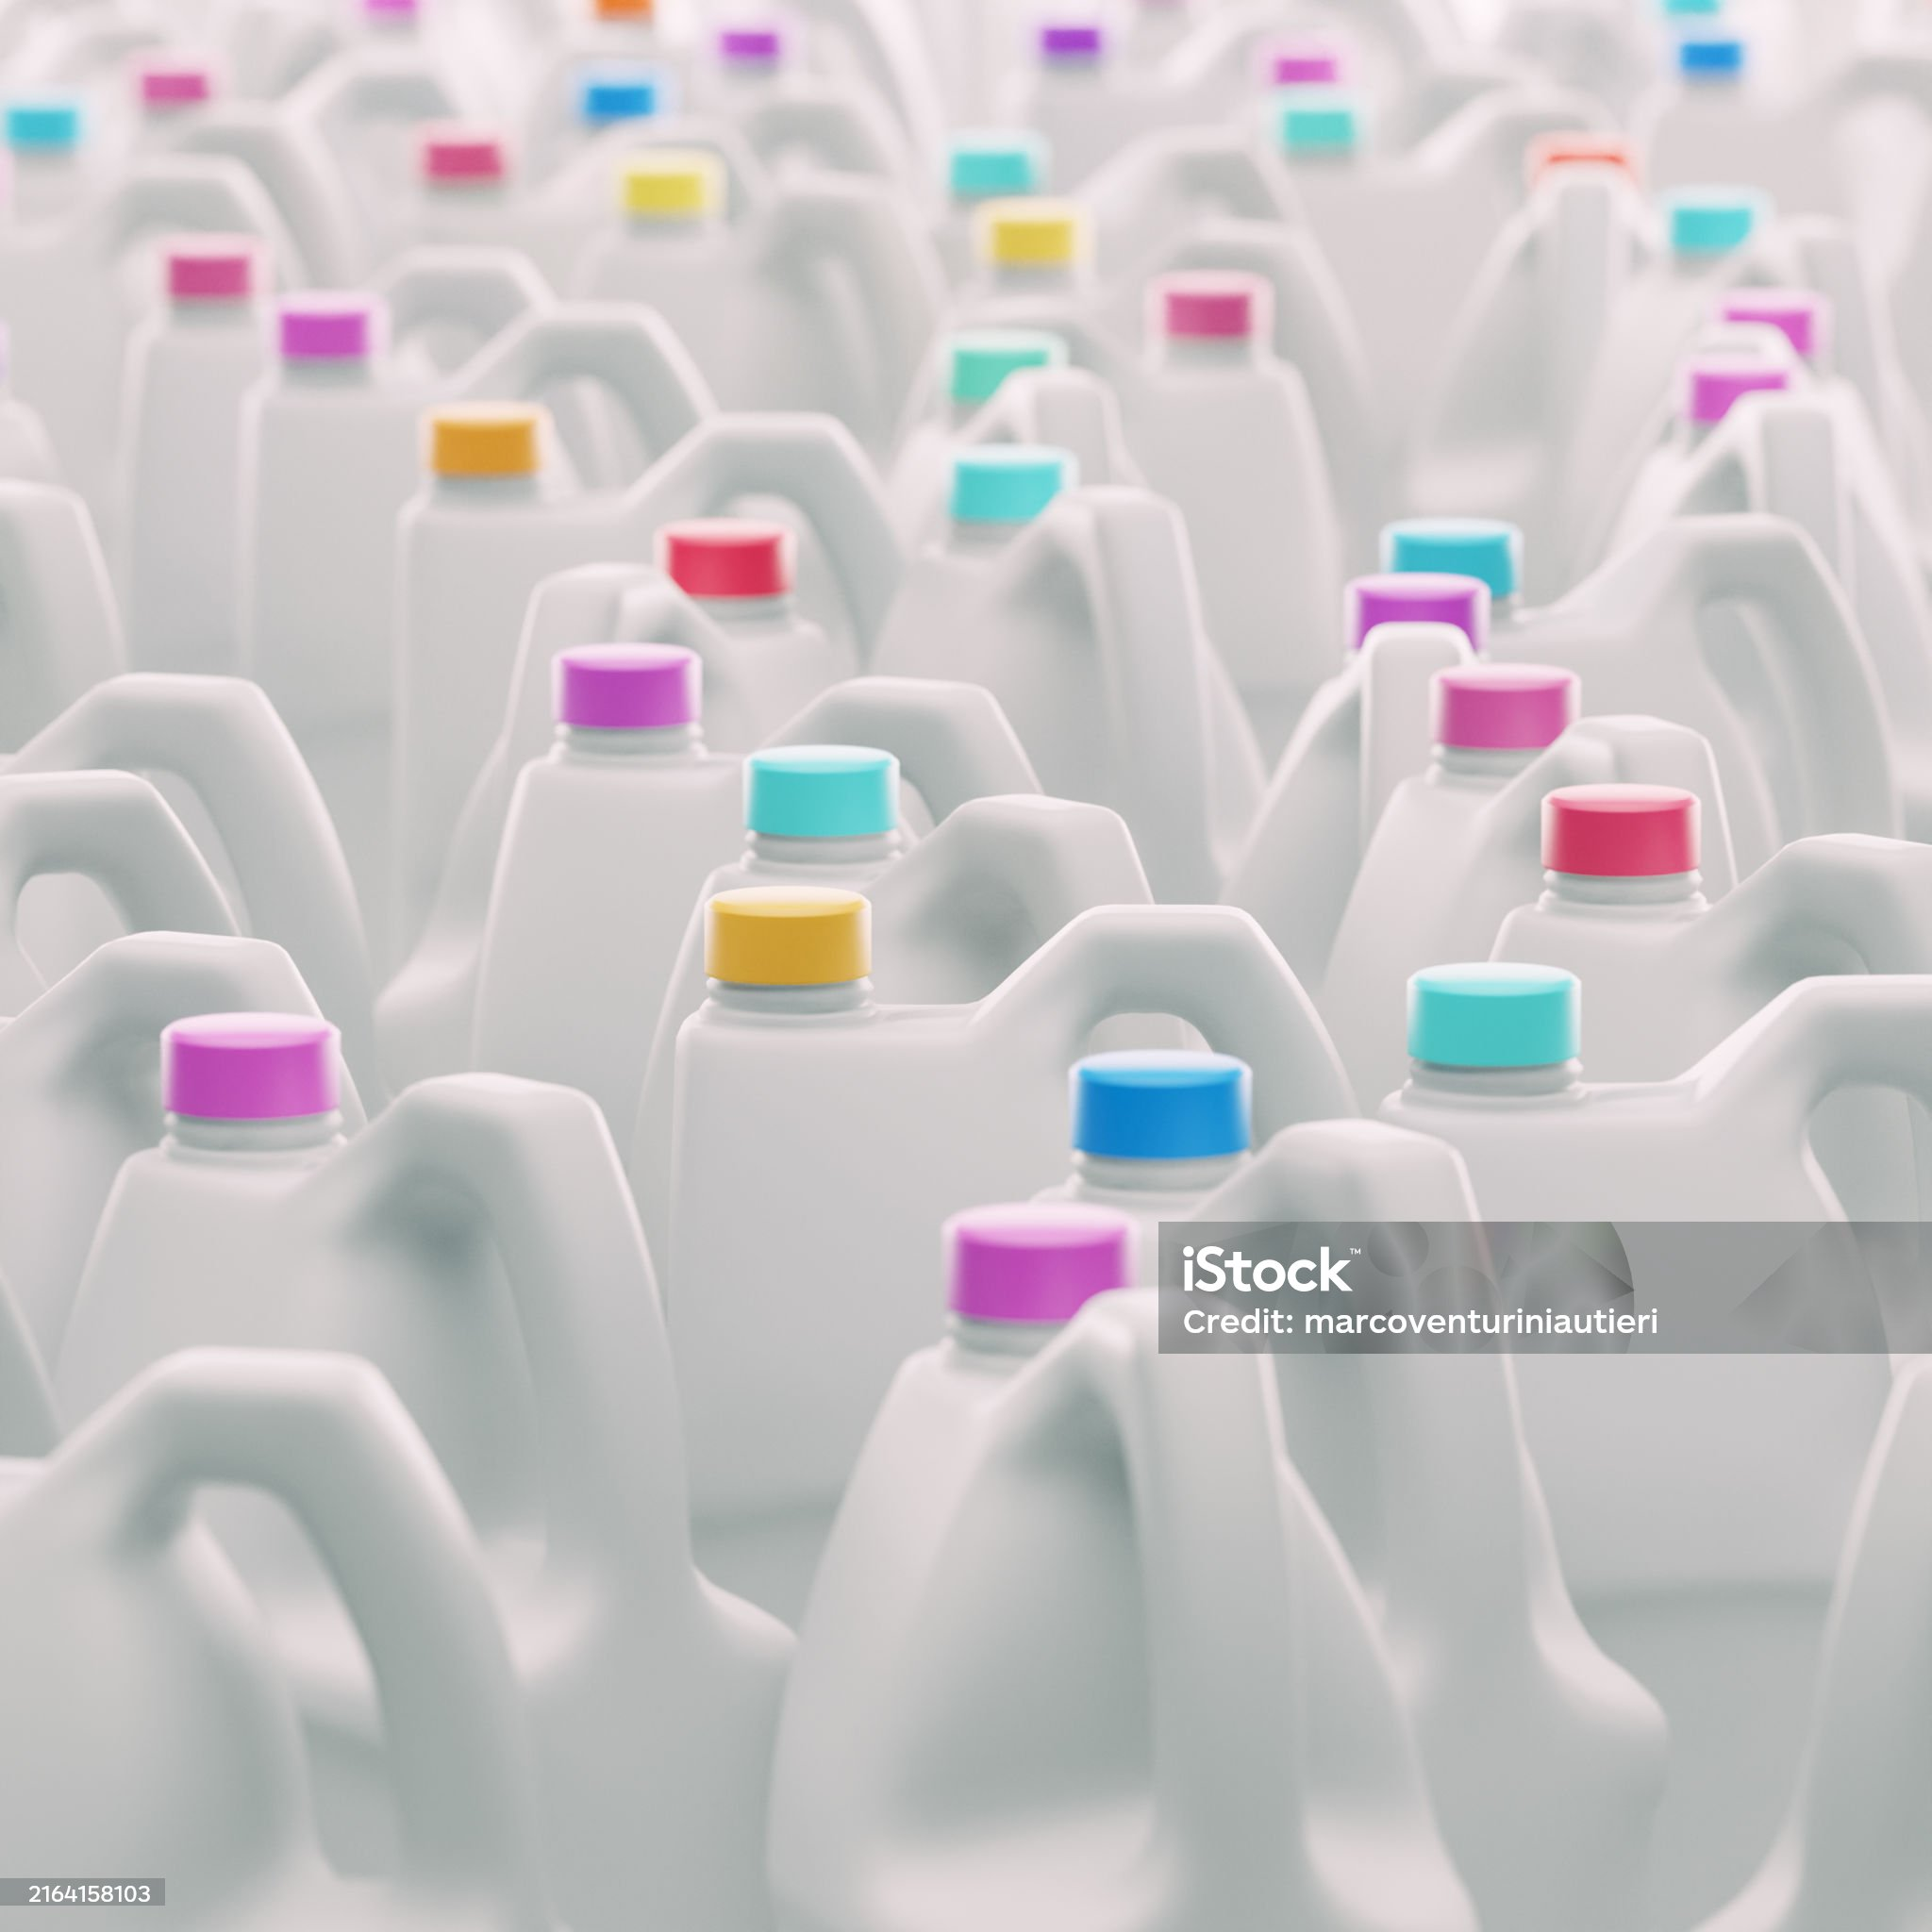
\includegraphics[width=.7\textwidth]{assets/example-image}

    \vfill

    % University and date information at the bottom of the titlepage.
    % Eastern Washington University \\
    \rule{.7\textwidth}{1pt}

    \vspace*{.25cm}

    \Large \today

    \rule{.7\textwidth}{1pt}

\end{titlepage}

\noindent\textbf{1:}

\section{Code example using \texttt{listings} package}

\begin{lstlisting}[language=Java]
public class HelloWorld {
    public static void main(String[] args) {
        System.out.println("Hello, World!");
    }
}
\end{lstlisting}

\section{List example using \texttt{enumitem} package}

\begin{enumerate}[label=\roman*.]
    \item First item
    \item Second item
    \item Third item
\end{enumerate}

\section{Figure example using \texttt{subfigure} package}

\begin{figure}[!ht]
    \centering
    \subfigure[Subfigure 1]{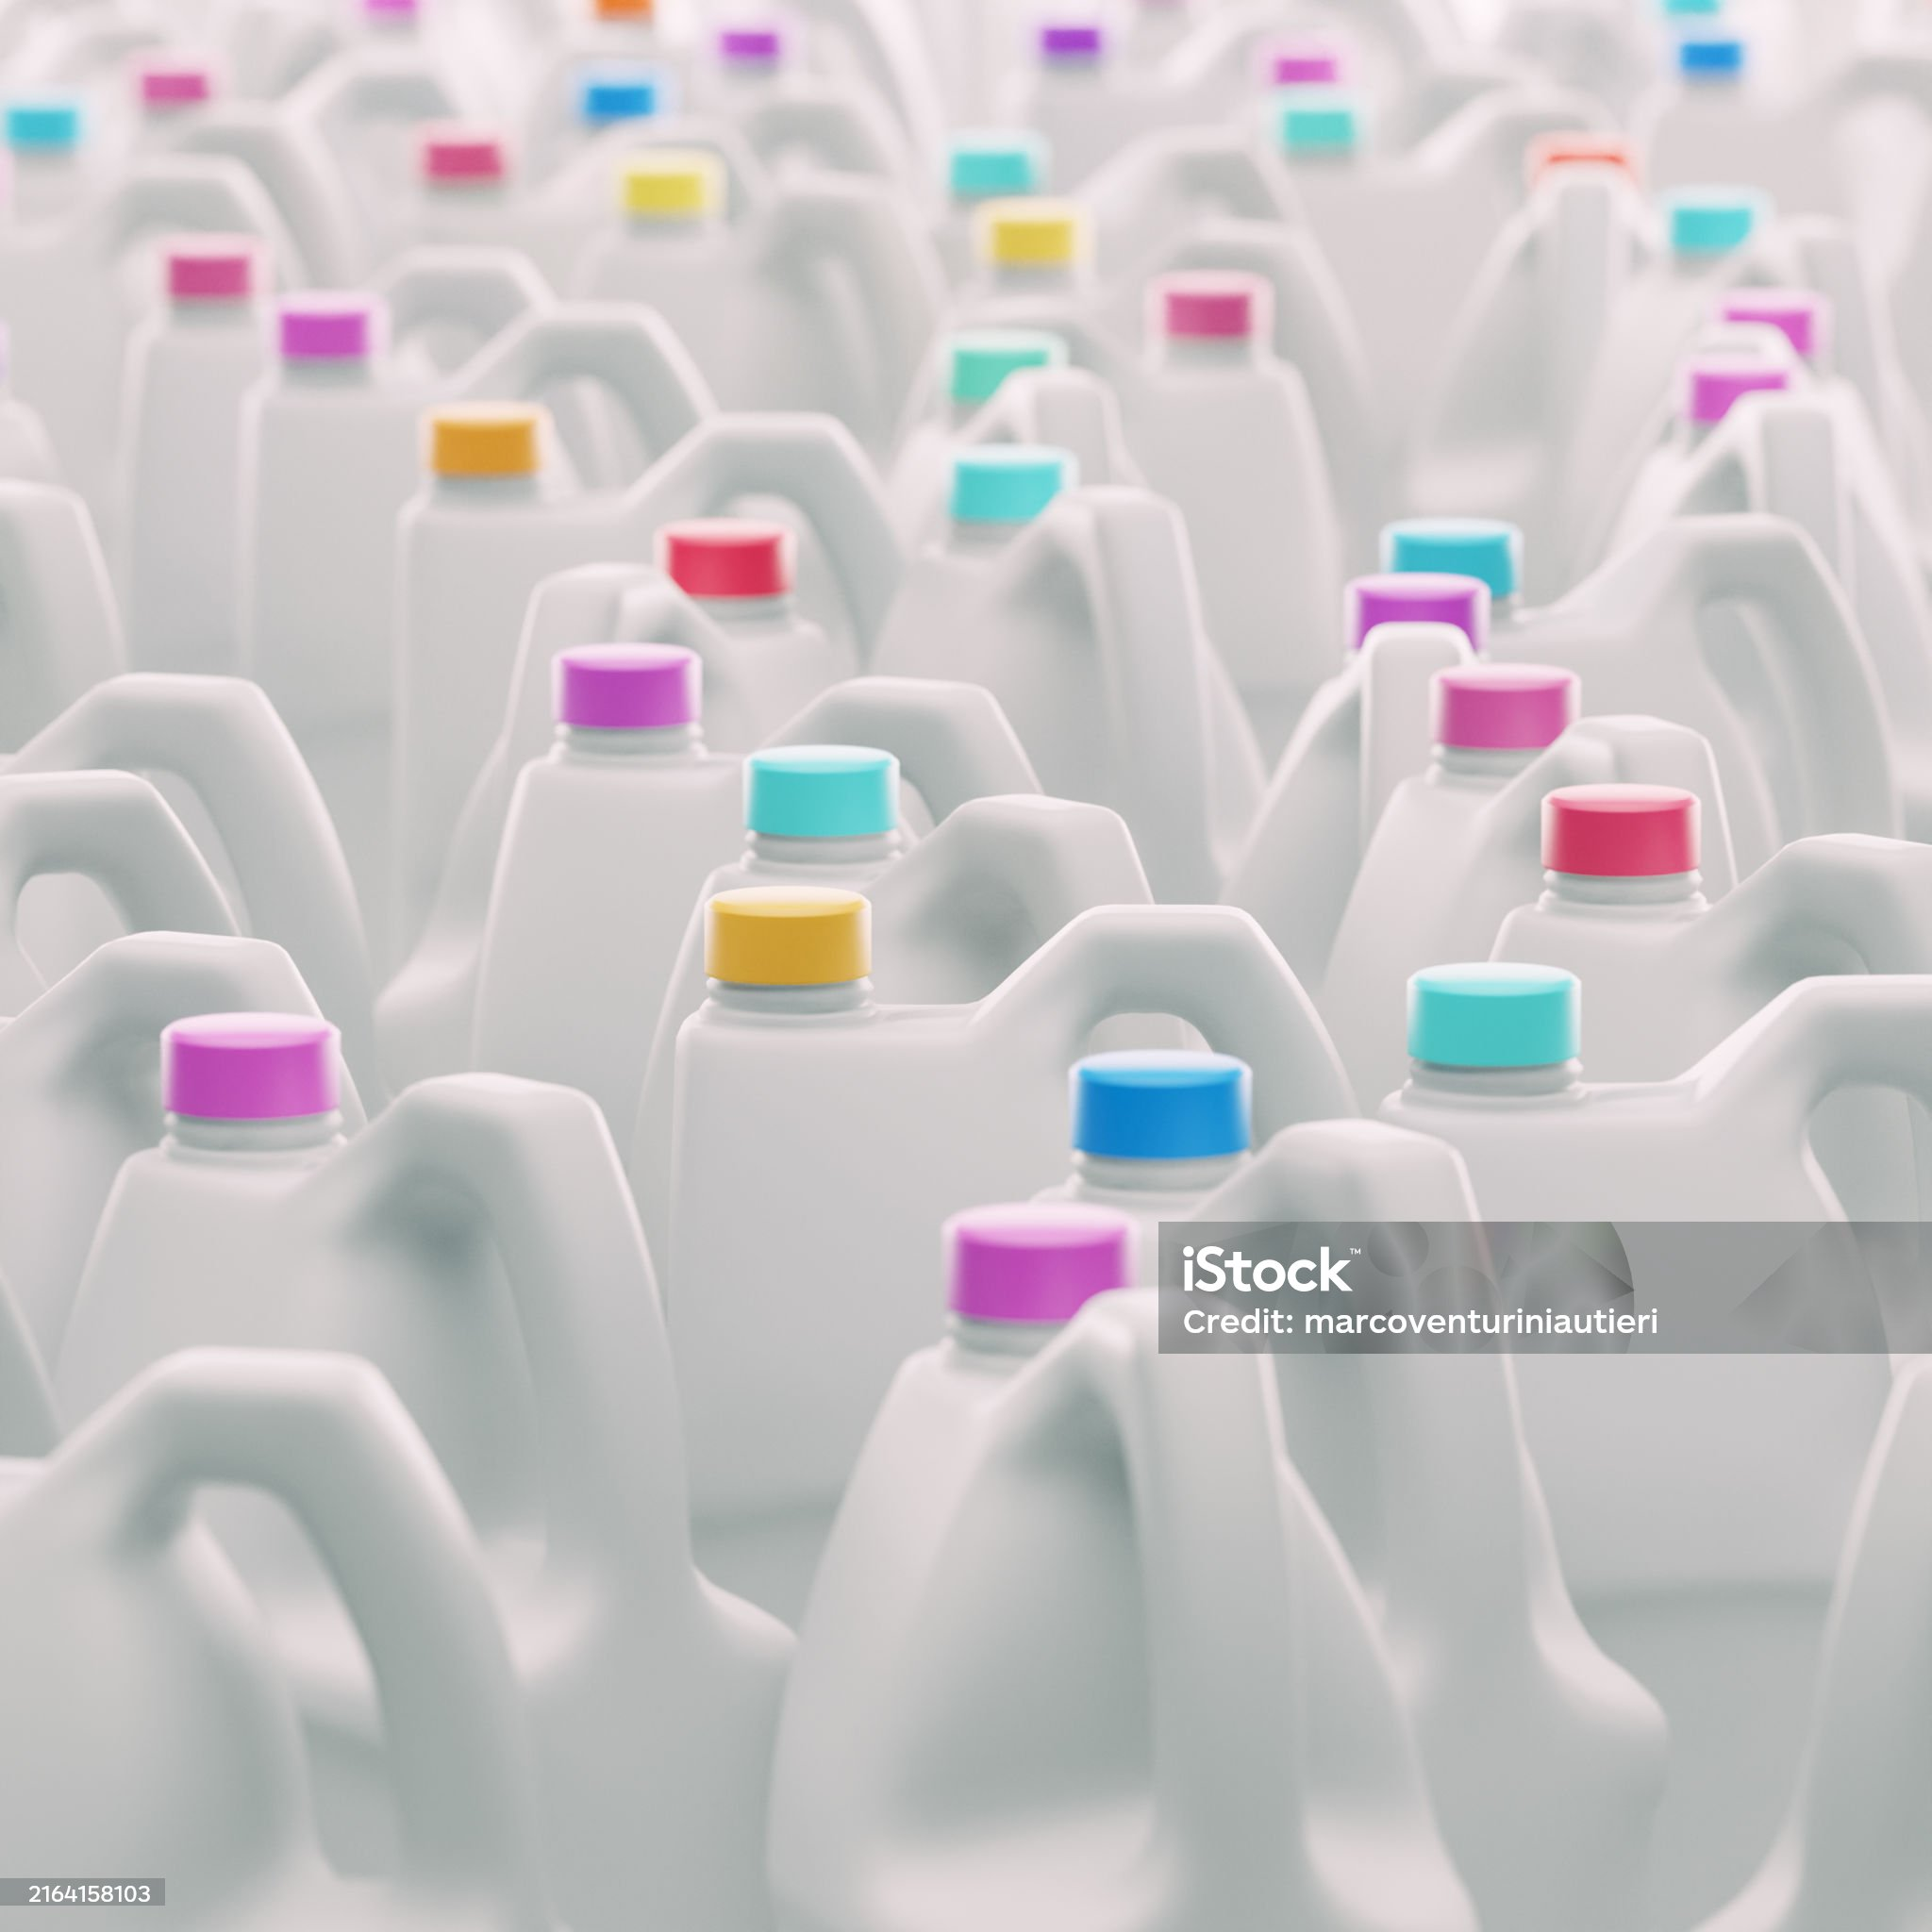
\includegraphics[width=0.45\textwidth]{assets/example-image.jpg}}
    \subfigure[Subfigure 2]{
\includegraphics[width=0.45\textwidth]{assets/example-image-2.jpg}}
    \caption{Caption for the subfigures.}
\end{figure}

\vspace{5mm}\noindent\textbf{2:}

\section{Example of \texorpdfstring{\texttt{cprotect}}{cprotect} Usage}

\cprotect\subsection{Using \texorpdfstring{\protect\texttt{cprotect}}{cprotect} in Section Titles}

Sometimes, you may want to include special characters or commands in section titles. For example, the following section title includes a LaTeX command:

\cprotect\subsubsection{Displaying \protect\texttt{\textbackslash texttt\{cprotect\}} in a Section Title}

\cprotect\subsection{Using \protect\texttt{cprotect} in Captions}

You can also use \texttt{cprotect} to include special characters or commands in figure or table captions. Here is an example:

\begin{figure}[!ht]
    \centering
    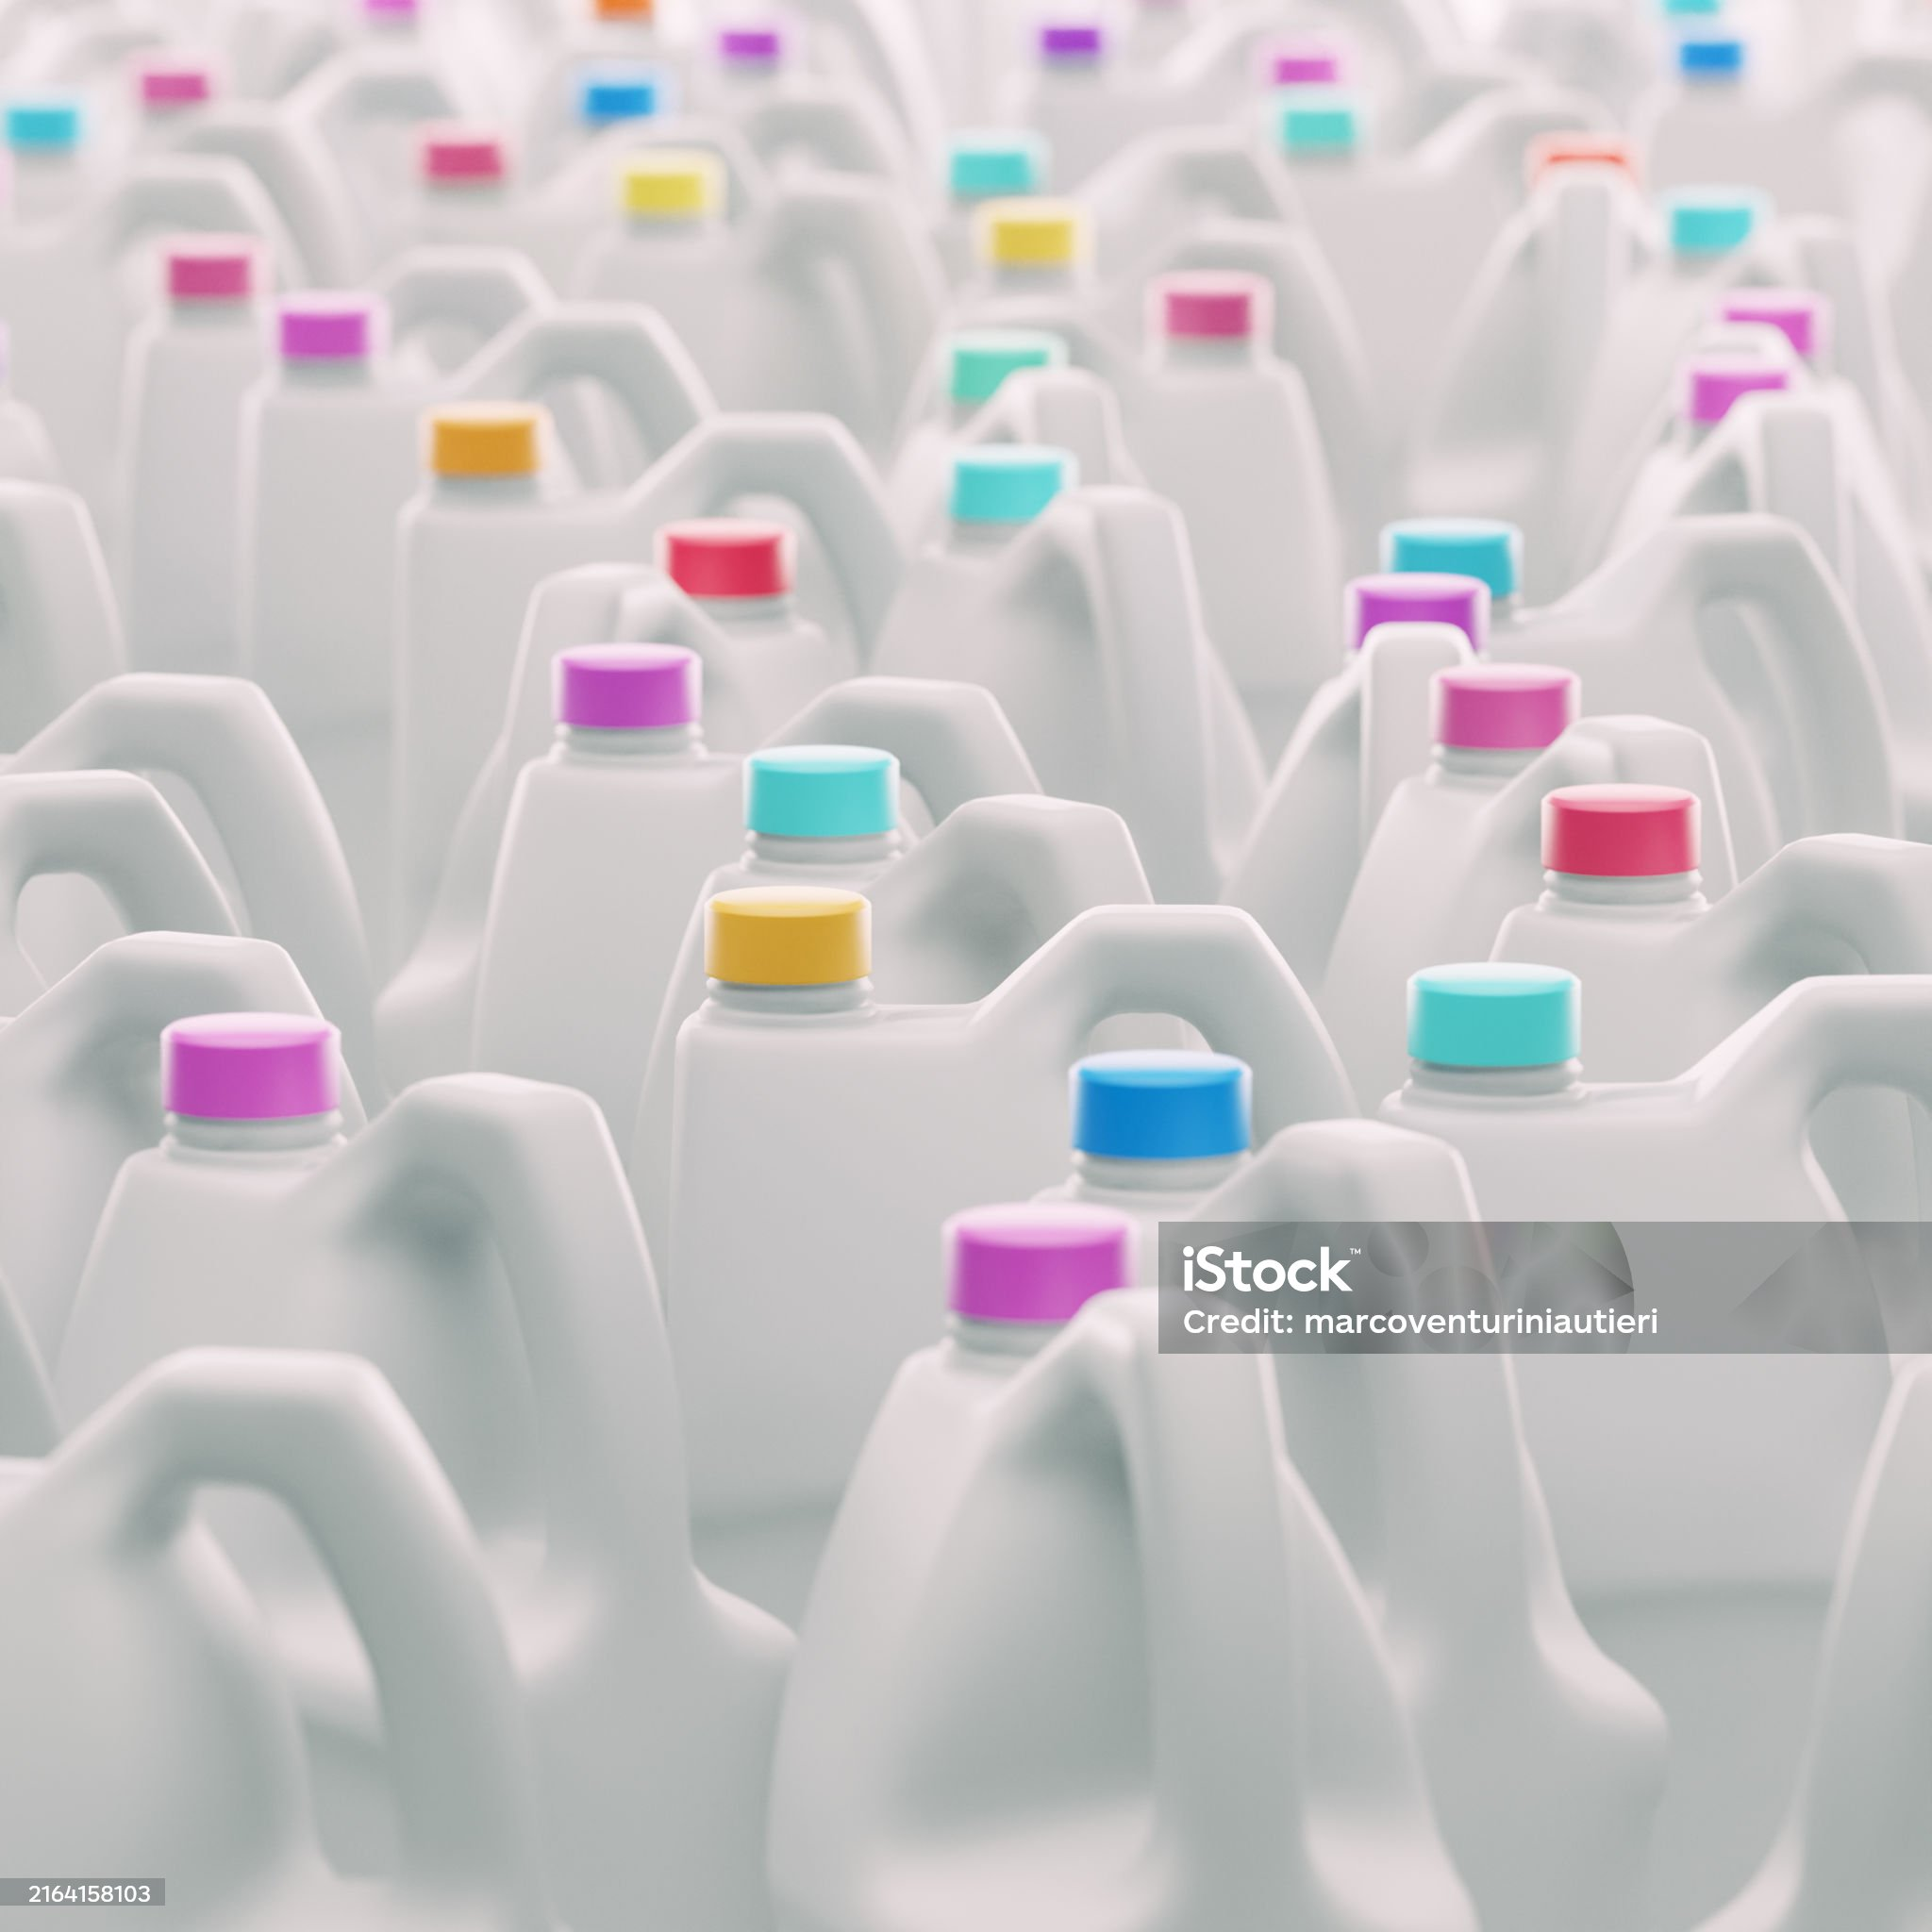
\includegraphics[width=0.5\textwidth]{assets/example-image.jpg}
    \cprotect\caption{This is a caption with a LaTeX command: \texttt{\textbackslash texttt\{cprotect\}}}
\end{figure}

\section{Example of \texorpdfstring{\texttt{xcolor}}{xcolor} Usage in Code Listings}

\begin{lstlisting}[language=TeX]
    \definecolor{codegreen}{rgb}{0,0.6,0}
    \definecolor{codegray}{rgb}{0.5,0.5,0.5}
    \definecolor{codepurple}{rgb}{0.58,0,0.82}
    \definecolor{backcolour}{rgb}{0.95,0.95,0.92}
    
    \lstdefinestyle{mystyle}{
        backgroundcolor=\color{backcolour},   
        commentstyle=\color{codegreen},
        keywordstyle=\color{magenta},
        numberstyle=\tiny\color{codegray},
        stringstyle=\color{codepurple},
        basicstyle=\ttfamily\footnotesize,
        breakatwhitespace=false,         
        breaklines=true,                 
        captionpos=b,                    
        keepspaces=true,                 
        numbers=left,                    
        numbersep=5pt,                  
        showspaces=false,                
        showstringspaces=false,
        showtabs=false,                  
        tabsize=2
    }
    
    \lstset{style=mystyle} 
\end{lstlisting}

\vspace{5mm}\textit{c.}

\section{Example of \texttt{amsmath} Package Usage}e

The \texttt{amsmath} package provides various features to display mathematical expressions. Here are some examples:

\subsection{Aligning Equations}

The \texttt{align} environment allows you to align equations at the equal sign or any other character:

\begin{align}
    a + b &= c \\
    d + e &= f
\end{align}

\subsection{Matrices}

The \texttt{bmatrix} environment allows you to create matrices with brackets:

\[
\mathbf{A} = \begin{bmatrix}
    a & b \\
    c & d
\end{bmatrix}
\]

\subsection{Cases}

The \texttt{cases} environment is useful for piecewise-defined functions:

\[
f(x) = \begin{cases} 
    x^2 & \text{if } x \geq 0 \\
    -x & \text{if } x < 0 
\end{cases}
\]

\subsection{Fractions}

You can use the \texttt{\textbackslash frac} command to create fractions:

\[
\frac{a}{b}
\]

\subsection{Multiline Equations}

The \texttt{multline} environment allows you to break long equations into multiple lines:

\begin{multline}
    a + b + c + d + e + f + g + h + i + j + k + l + m + n + o + p + q + r + s + t + u + v + w + x + y + z \\
    = 1 + 2 + 3 + 4 + 5 + 6 + 7 + 8 + 9 + 10 + 11 + 12 + 13 + 14 + 15 + 16 + 17 + 18 + 19 + 20 + 21 + 22 + 23 + 24 + 25 + 26
\end{multline}

\vspace{5mm}\textit{d.}

\section{Example of \texttt{amssymb} Package Usage}

The \texttt{amssymb} package provides various additional mathematical symbols. Here are some examples:

\subsection{Set Notations}

\[
\mathbb{N} \quad \mathbb{Z} \quad \mathbb{Q} \quad \mathbb{R} \quad \mathbb{C}
\]

\subsection{Logic Symbols}

\[
\forall \quad \exists \quad \neg \quad \wedge \quad \vee \quad \Rightarrow \quad \Leftrightarrow
\]

\subsection{Other Symbols}

\[
\hbar \quad \ell \quad \imath \quad \jmath \quad \Box \quad \Diamond \quad \aleph \quad \beth
\]

\section{Example of \texttt{pdfpages} Package Usage}

The \texttt{pdfpages} package allows you to include pages from external PDF documents into your LaTeX document. Here is an example:


\includepdf[pages=1-2]{./sample.pdf}

In this example, the first two pages of the PDF file located at \texttt{./sample.pdf} are included in the document.


\section{Example of \texttt{hyperref} Package Usage}

The \texttt{hyperref} package allows you to create hyperlinks within your document, as well as to external URLs. Here are some examples:

\subsection{Internal Links}

You can create internal links to sections, figures, tables, etc. For example, here is a link to the section on \hyperref[sec:code-example]{Code Example}.

\subsection{External Links}

You can also create links to external websites. For example, here is a link to \href{https://www.latex-project.org/}{LaTeX Project}.

\subsection{Customizing Links}

You can customize the appearance of links using the \texttt{hypersetup} command. For example:

\hypersetup{
    colorlinks=true,
    linkcolor=blue,
    filecolor=magenta,      
    urlcolor=cyan,
}

With these settings, internal links will be blue, file links will be magenta, and URL links will be cyan.

\subsection{Link to a Figure}

Here is a link to \hyperref[fig:example]{Figure 1}.

\begin{figure}[!ht]
    \centering
    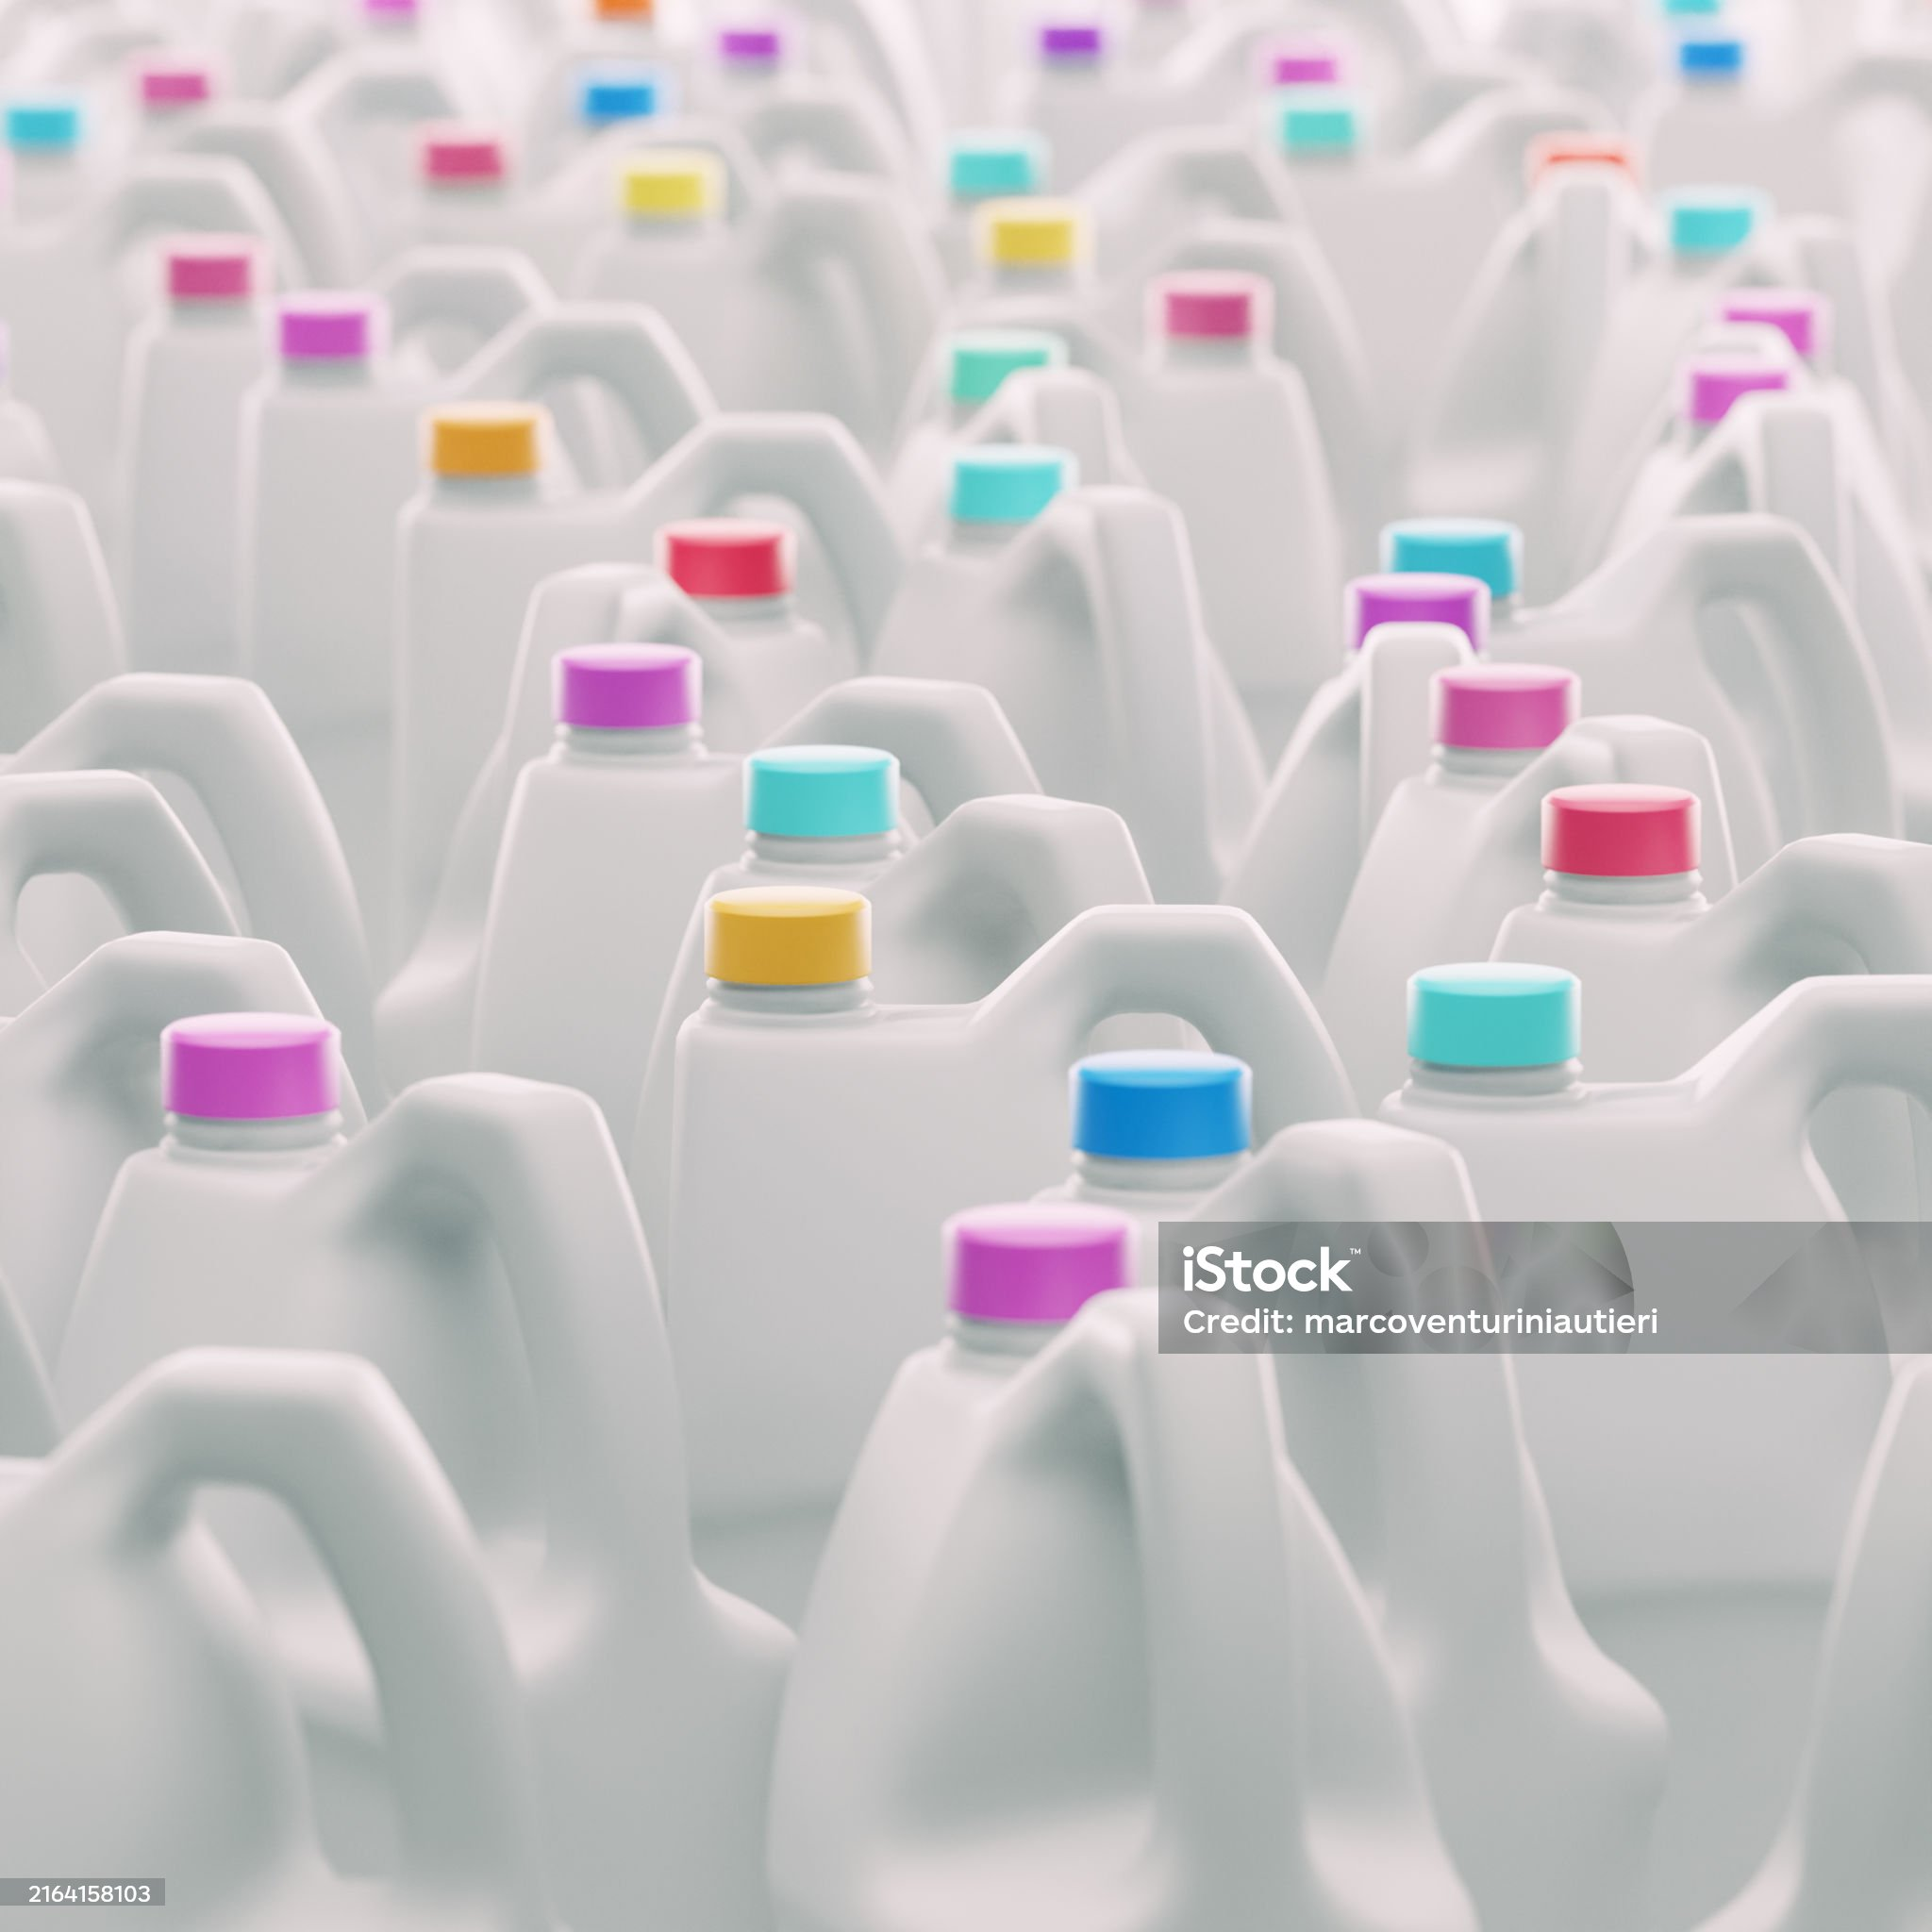
\includegraphics[width=0.5\textwidth]{assets/example-image.jpg}
    \caption{Example image}
    \label{fig:example}
\end{figure}

\section{Example of \texttt{graphicx} Package Usage}

The \texttt{graphicx} package allows you to include images in your document. Here is an example:

\begin{figure}[!ht]
    \centering
    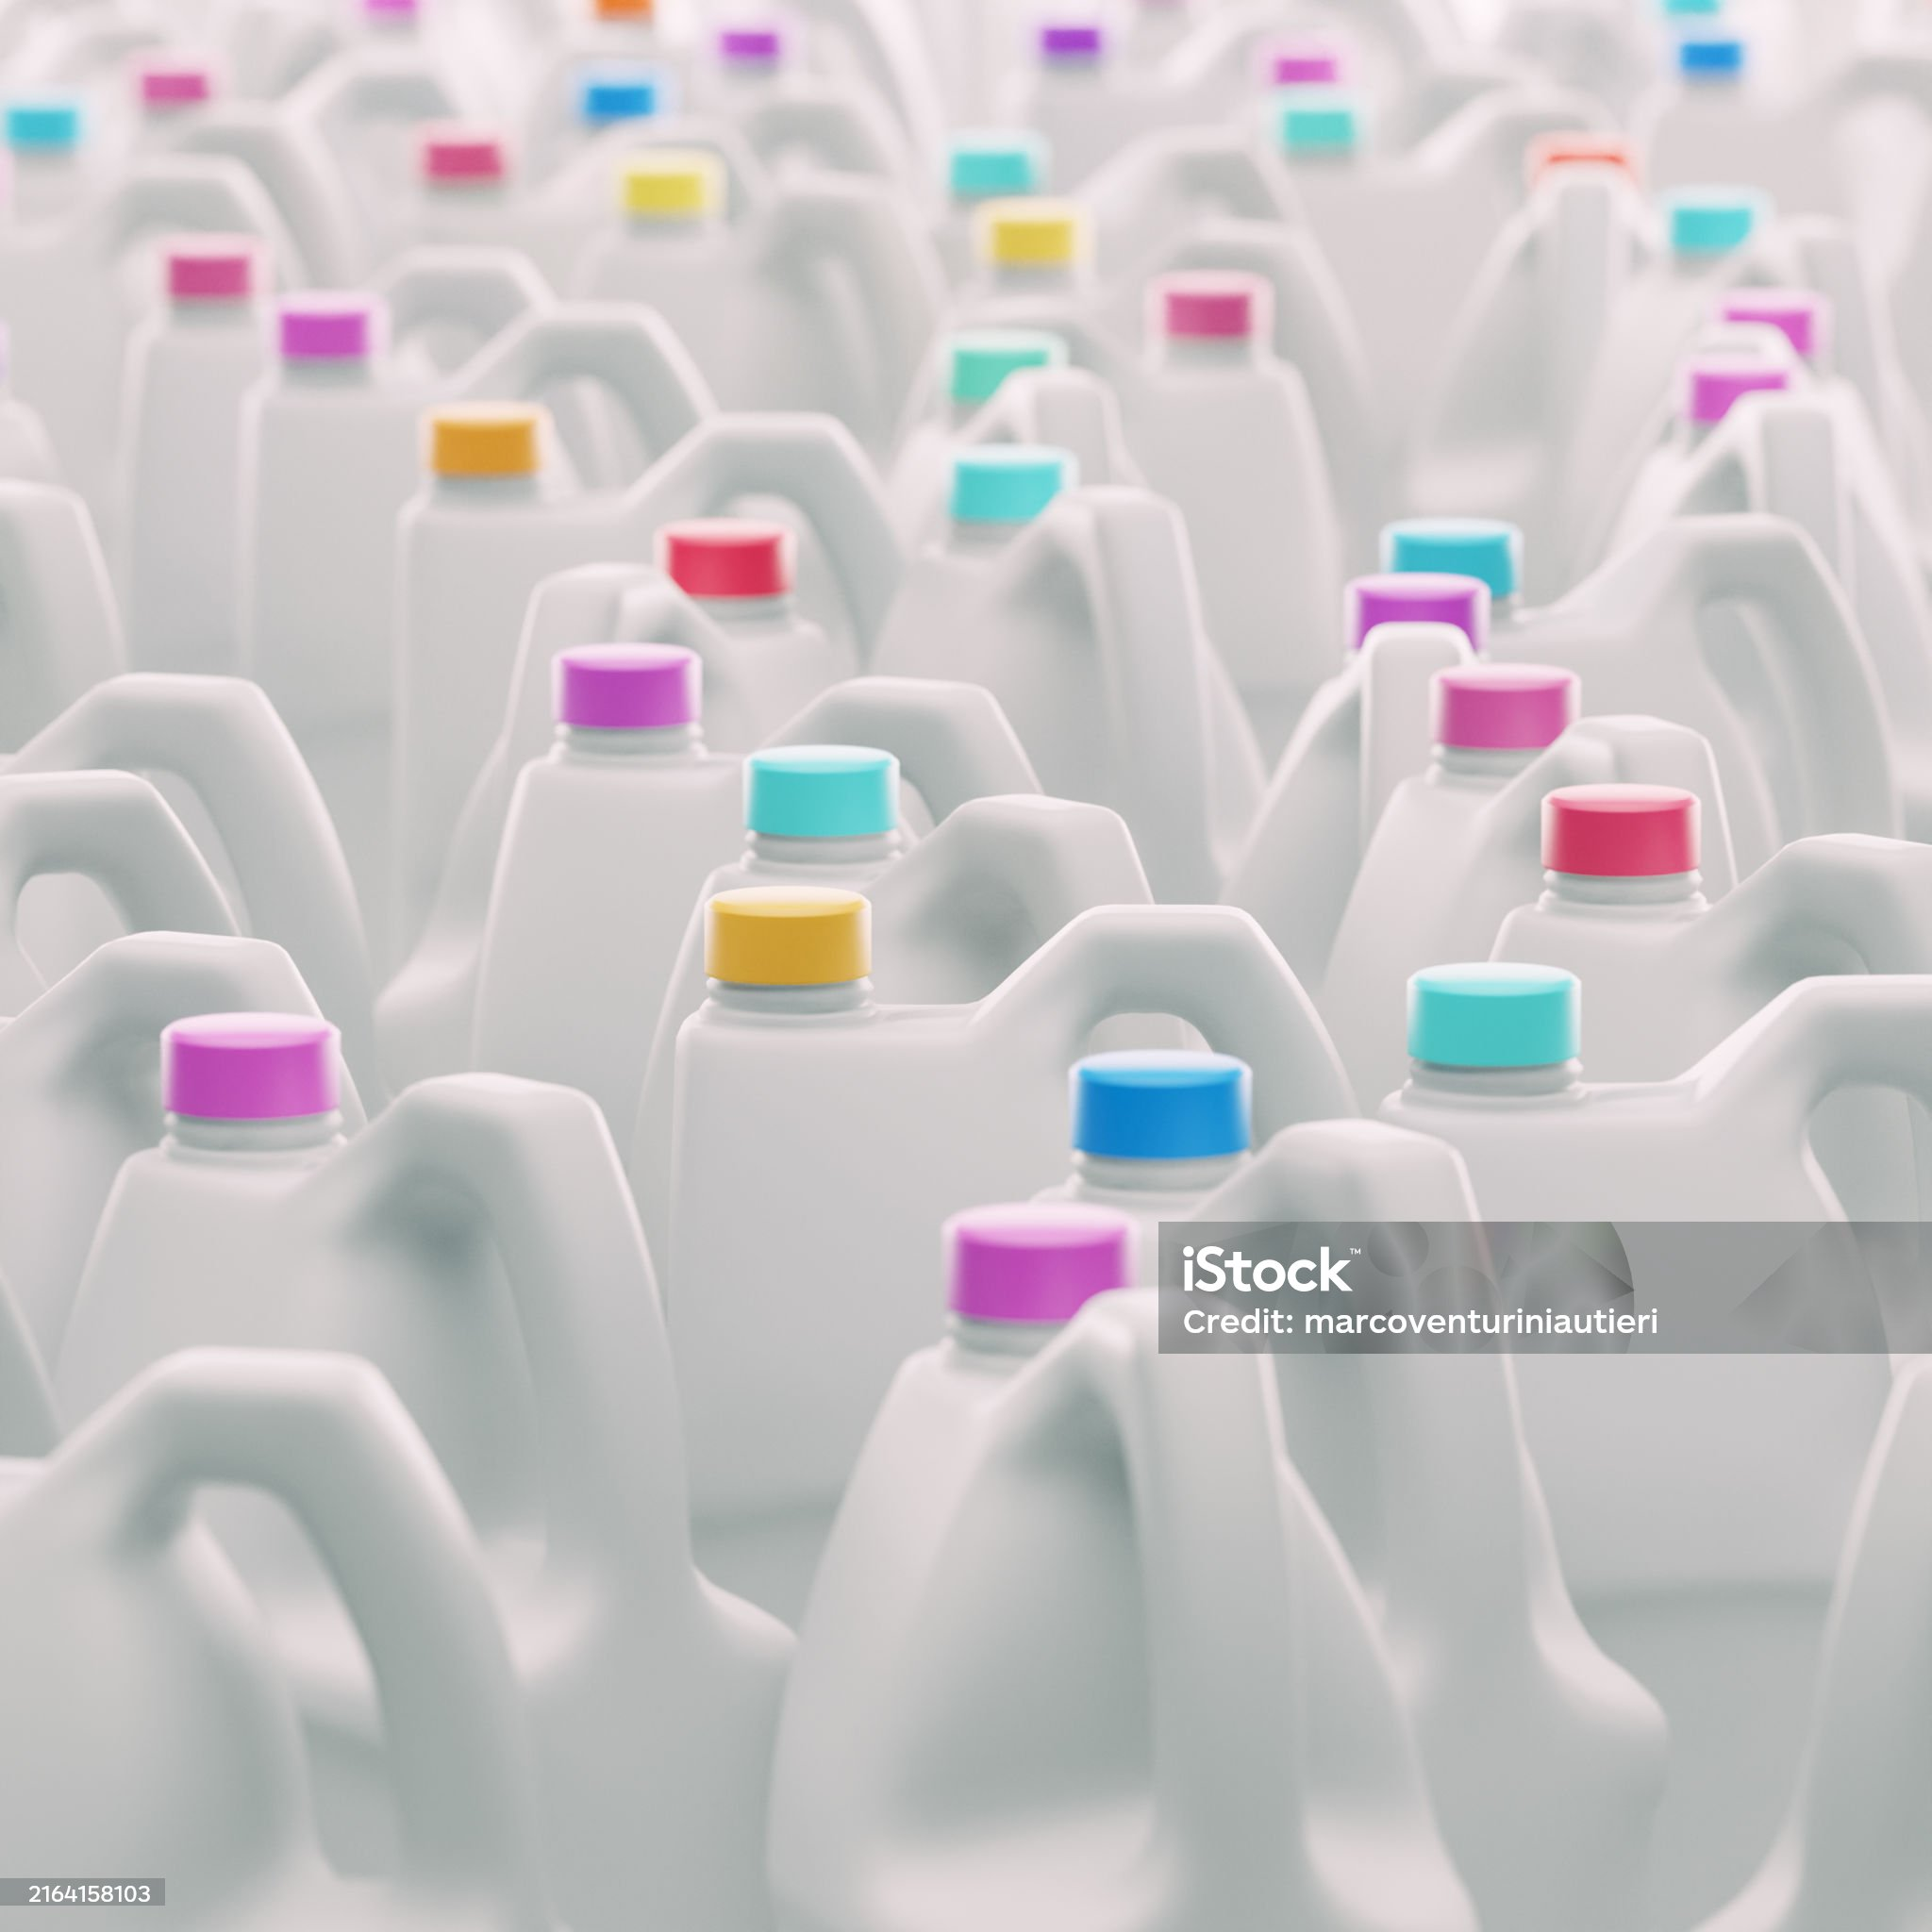
\includegraphics[width=0.5\textwidth]{assets/example-image.jpg}
    \caption{Example image included using the \texttt{graphicx} package}
    \label{fig:graphicx-example}
\end{figure}

\end{document}
